\documentclass[journal,12pt,twocolumn]{IEEEtran}

\usepackage{setspace}
\usepackage{gensymb}
\singlespacing
\usepackage[cmex10]{amsmath}
\usepackage{multirow}
\usepackage{amsthm}
\usepackage{mathrsfs}
\usepackage{txfonts}
\usepackage{stfloats}
\usepackage{bm}
\usepackage{cite}
\usepackage{cases}
\usepackage{subfig}

\usepackage{longtable}

\usepackage{enumitem}
\usepackage{mathtools}
\usepackage{steinmetz}
\usepackage{tikz}
\usepackage{circuitikz}
\usepackage{verbatim}
\usepackage{tfrupee}
\usepackage[breaklinks=true]{hyperref}
\usepackage{graphicx}
\usepackage{tkz-euclide}

\usetikzlibrary{calc,math}
\usepackage{listings}
    \usepackage{color}                                            %%
    \usepackage{array}                                            %%
    \usepackage{longtable}                                        %%
    \usepackage{calc}                                             %%
    \usepackage{multirow}                                         %%
    \usepackage{hhline}                                           %%
    \usepackage{ifthen}                                           %%
    \usepackage{lscape}     
\usepackage{multicol}
\usepackage{chngcntr}

\DeclareMathOperator*{\Res}{Res}

\renewcommand\thesection{\arabic{section}}
\renewcommand\thesubsection{\thesection.\arabic{subsection}}
\renewcommand\thesubsubsection{\thesubsection.\arabic{subsubsection}}

\renewcommand\thesectiondis{\arabic{section}}
\renewcommand\thesubsectiondis{\thesectiondis.\arabic{subsection}}
\renewcommand\thesubsubsectiondis{\thesubsectiondis.\arabic{subsubsection}}


\hyphenation{op-tical net-works semi-conduc-tor}
\def\inputGnumericTable{}                                 %%

\lstset{
%language=C,
frame=single, 
breaklines=true,
columns=fullflexible
}
\graphicspath{{./Figures/}}
\begin{document}


\newtheorem{theorem}{Theorem}[section]
\newtheorem{problem}{Problem}
\newtheorem{proposition}{Proposition}[section]
\newtheorem{lemma}{Lemma}[section]
\newtheorem{corollary}[theorem]{Corollary}
\newtheorem{example}{Example}[section]
\newtheorem{definition}[problem]{Definition}

\newcommand{\BEQA}{\begin{eqnarray}}
\newcommand{\EEQA}{\end{eqnarray}}
\newcommand{\define}{\stackrel{\triangle}{=}}
\bibliographystyle{IEEEtran}
\raggedbottom
\setlength{\parindent}{0pt}
\providecommand{\mbf}{\mathbf}
\providecommand{\pr}[1]{\ensuremath{\Pr\left(#1\right)}}
\providecommand{\qfunc}[1]{\ensuremath{Q\left(#1\right)}}
\providecommand{\sbrak}[1]{\ensuremath{{}\left[#1\right]}}
\providecommand{\lsbrak}[1]{\ensuremath{{}\left[#1\right.}}
\providecommand{\rsbrak}[1]{\ensuremath{{}\left.#1\right]}}
\providecommand{\brak}[1]{\ensuremath{\left(#1\right)}}
\providecommand{\lbrak}[1]{\ensuremath{\left(#1\right.}}
\providecommand{\rbrak}[1]{\ensuremath{\left.#1\right)}}
\providecommand{\cbrak}[1]{\ensuremath{\left\{#1\right\}}}
\providecommand{\lcbrak}[1]{\ensuremath{\left\{#1\right.}}
\providecommand{\rcbrak}[1]{\ensuremath{\left.#1\right\}}}
\theoremstyle{remark}
\newtheorem{rem}{Remark}
\newcommand{\sgn}{\mathop{\mathrm{sgn}}}
\providecommand{\abs}[1]{\left\vert#1\right\vert}
\providecommand{\res}[1]{\Res\displaylimits_{#1}} 
\providecommand{\norm}[1]{\left\lVert#1\right\rVert}
%\providecommand{\norm}[1]{\lVert#1\rVert}
\providecommand{\mtx}[1]{\mathbf{#1}}
\providecommand{\mean}[1]{E\left[ #1 \right]}
\providecommand{\fourier}{\overset{\mathcal{F}}{ \rightleftharpoons}}
%\providecommand{\hilbert}{\overset{\mathcal{H}}{ \rightleftharpoons}}
\providecommand{\system}{\overset{\mathcal{H}}{ \longleftrightarrow}}
	%\newcommand{\solution}[2]{\textbf{Solution:}{#1}}
\newcommand{\solution}{\noindent \textbf{Solution: }}
\newcommand{\cosec}{\,\text{cosec}\,}
\providecommand{\dec}[2]{\ensuremath{\overset{#1}{\underset{#2}{\gtrless}}}}
\newcommand{\myvec}[1]{\ensuremath{\begin{pmatrix}#1\end{pmatrix}}}
\newcommand{\mydet}[1]{\ensuremath{\begin{vmatrix}#1\end{vmatrix}}}
\newcommand*{\permcomb}[4][0mu]{{{}^{#3}\mkern#1#2_{#4}}}
\newcommand*{\perm}[1][-3mu]{\permcomb[#1]{P}}
\newcommand*{\comb}[1][-1mu]{\permcomb[#1]{C}}
\numberwithin{equation}{subsection}
\makeatletter
\@addtoreset{figure}{problem}
\makeatother
\let\StandardTheFigure\thefigure
\let\vec\mathbf
\renewcommand{\thefigure}{\theproblem}
\def\putbox#1#2#3{\makebox[0in][l]{\makebox[#1][l]{}\raisebox{\baselineskip}[0in][0in]{\raisebox{#2}[0in][0in]{#3}}}}
     \def\rightbox#1{\makebox[0in][r]{#1}}
     \def\centbox#1{\makebox[0in]{#1}}
     \def\topbox#1{\raisebox{-\baselineskip}[0in][0in]{#1}}
     \def\midbox#1{\raisebox{-0.5\baselineskip}[0in][0in]{#1}}
\vspace{3cm}
\title{Assignment 4}
\author{Sujal - AI20BTECH11020}
\maketitle
\newpage
\bigskip
\renewcommand{\thefigure}{\theenumi}
\renewcommand{\thetable}{\theenumi}
Download all latex codes from 

\begin{lstlisting}
https://github.com/https://github.com/sujal100/EE3900/blob/main/Assignment4/Assignment4.tex
\end{lstlisting}

Download all python codes from 

\begin{lstlisting}
https://github.com/https://github.com/sujal100/EE3900/blob/main/Assignment4/codes/code.py
\end{lstlisting}
\section{Problem}
(Linear forms Q-2.22) Find the shortest distance between the lines 
\begin{align}
\frac{x+1}{7} = \frac{y+1}{-6} &= \frac{z+1}{1}, 
\\
\frac{x-3}{1} = \frac{y-5}{-2} &= \frac{z-7}{1} 
\end{align}

\section{Solution}
In the given  problem
\begin{align}
\vec{A}_1= \myvec{-1\\-1\\-1}, \vec{m}_1=\myvec{7 \\ -6 \\1},
\vec{A}_2= \myvec{3\\5\\7}, \vec{m}_2 =\myvec{1 \\ -2 \\1}.
\end{align}
The lines will intersect if
\begin{align}
\myvec{-1\\-1\\-1} + \lambda_1\myvec{7 \\ -6 \\1}
= \myvec{3\\5\\7} + \lambda_2\myvec{1 \\ -2 \\1}
\\
\implies \lambda_1\myvec{7 \\ -6 \\1} - \lambda_2\myvec{1 \\ -2 \\1} &= \myvec{3\\5\\7}-\myvec{-1\\-1\\-1}  
\\
\implies \myvec{7 & 1 \\ -6 & -2 \\ 1 & 1}\myvec{\lambda_1\\ \lambda_2} = \myvec{4\\6\\8}
\end{align}
Row reducing the augmented matrix,
\begin{align}
\myvec{
7 & 1 & 4 
\\
-6 & -2 & 6
\\
1 & 1 & 8
}
\xleftrightarrow[]{R_3\leftrightarrow R_1}
\myvec{
1 & 1 & 8
\\
-6 & -2 & 6
\\
7 & 1 & 4
}
\\
\xleftrightarrow[]{\substack{R_2= 6R_1+R_2\\R_3 = -7R_1+R_3}}
\myvec{
1 & 1 & 8
\\
0 & 4 & 54
\\
0 & -6 & -52
}
\xleftrightarrow[]{R_2= \frac{R_2}{4}}
\myvec{
1 & 1 & 8
\\
0 & 1 & \frac{27}{2}
\\
0 & -6 & -52
}
\\
\xleftrightarrow[]{R_3=6R_2+R_3}
\myvec{
1 & 1 & 8
\\
0 & 1 & \frac{27}{2}
\\
0 & 0 & 29
}
\end{align}
The above matrix has $rank = 3$.  Hence, the lines do not intersect.  Note that the lines are not parallel but they  lie on parallel planes.  Such lines are known as {\em skew} lines as can be seen in Fig \ref{skew_lines}.\\
$\therefore$ The distance between given two lines is 
\begin{align}
\frac{\abs{\brak{\vec{A}_2-\vec{A}_1}^T\brak{\vec{m}_1\times\vec{m}_2}}}{\norm{\vec{m}_1\times\vec{m}_2}} = 10.77
\end{align}
\begin{figure}[!ht]
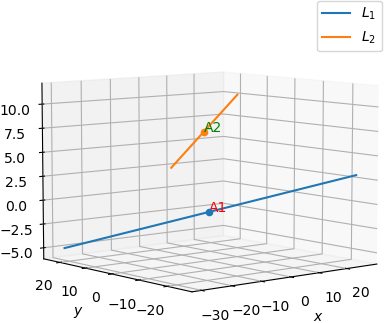
\includegraphics[width=\columnwidth]{plot.png}
\caption{plot of lines}
\label{skew_lines}
\end{figure}
\end{document}